\section{Defining Impact of External Queries}
\label{sec:analysis:exposing_interference}
This section looks at how external queries interfere with caches and,
consequently, with instructions using these caches. The results of the analyses
performed in this section are not likely to be of direct interest to the user,
since they have little control over queries themselves. However, this section
introduces the concepts that define the interference generated by cache
coherence and the analysis of queries is key to the more exploitable results
of Section~\ref{sec:analysis:missing_link}.

The characterization of the effects of each query on a cache provides
information about what causes an instruction to result in a cache miss or to be
delayed (which is not observable in the analyses of
Section~\ref{sec:analysis:hit_and_miss}). In effect, two of the three proposed
categories of interference specify which permissions are lost, which correlates
to which instructions would miss if executed after the interference.

\subsection{Minor Interference}
\label{sec:analysis:minor_interference}
No handling of an event by a cache is instantaneous: every time a cache has to
process an incoming query, there is a very small amount of time during which it
cannot be used by its core. As a result, all external queries lead to some kind
of interference. This small delay being the least disruption that can be
caused. While the effect of each delay is so small as to be considered
negligible, their accumulation most definitely is not.  The name \textit{minor
interference} is proposed for this unavailability period.

\begin{definition}[Minor Interference]
\label{def:interference:minor}
Minor interference occurs whenever a cache becomes unavailable for core requests
because it is handling an external bus query, yet the handling of that query
had not effect.
\end{definition}
\begin{example}[Minor Interference]
Figure~\ref{fig:minor-interference} shows an example of minor interference. The
figure indicates the current coherence state of the memory element involved for
both caches, as well as their outgoing query queue. In that example, Cache2
has to process Cache1's \texttt{GetS} broadcast, despite that
message not requiring any reply or coherence state update from Cache2.
\begin{figure}[hbt!]
\begin{center}
\resizebox{0.7\linewidth}{!}{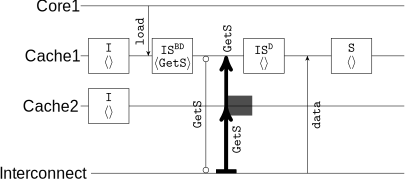
\includegraphics{\chapterdirectory/figure/load_seq_diagram_interference3_fixed.pdf}}
\end{center}
\caption{Minor Cache Coherence Interference}
\label{fig:minor-interference}
\end{figure}
\end{example}

Detection of this interference by the model is simply done by each cache
considering any observed external query as an occurrence of minor interference.
If the observed external query is later considered to be a different type of
interference, it is removed from the count of minor interferences.

For a minor cache coherence interference to be considered to have had an impact,
it must delay a request from a core. More specifically, the request has to
become available for transmission from the core to the cache, but the cache be
unavailable because it is already processing the interfering query. It is
considered as having an impact solely on that delayed instruction.

While counting the number of occurrences is easily done, detecting that a minor
interference had an impact on the program's execution would correspond to
detecting that a synchronization for either data or request with a cache
automaton (see Section~\ref{sec:model:cache}) could not be performed because
that automaton was in its $S_2$ location (waiting for the query handling time
to pass). Doing so might be possible, but requires numerous changes in the
model's automata, and is thus not currently supported. As a result, all
occurrences of minor interferences are counted, but the model does not let the
user know if they had an impact.

\subsection{Demoting Interference}
As explained in Section~\ref{sec:proper_cache_coherence_protocol}, cache
coherence protocols do not allow a cache to hold a memory element with writing
permissions while another cache holds that same memory element with reading
permissions. Thus, acquisition of a copy the memory element by another cache
leads to any cache currently holding it with writing permissions to lose them.
The name \textit{demoting interference} is proposed for this type of
interference.

\begin{definition}[Demoting Interference]
Demoting interference corresponds to the loss of writing permission for a memory
element by a cache because of an external query, while reading permissions are
kept.
\end{definition}


\begin{example}[Demoting Interference]
Figure~\ref{fig:demoting-interference} shows an example of
demoting interference: Cache2, receiving
a demand for read access on that memory element from Cache1, has to update the
value from the main memory and go from read-and-write permissions to read-only
permissions.

\begin{figure}[hbt!]
\begin{center}
\resizebox{0.7\linewidth}{!}{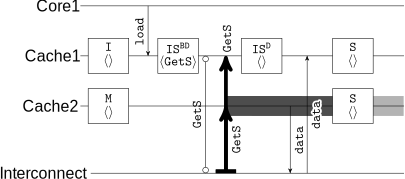
\includegraphics{\chapterdirectory/figure/load_when_modified_seq_diagram_interference3_fixed.pdf}}
\end{center}
\caption{Demoting Cache Coherence Interference}
\label{fig:demoting-interference}
\end{figure}
\end{example}

In order for a demoting interference to have had an impact, it must be followed
by a \storeinstr{} instruction, with any number of \loadinstr{} in-between, but
no \evictinstr{}. The demoting interference is only considered to have had an
impact on that \storeinstr{} instruction, not on the other instructions
in-between nor on future instructions.

To detect demoting interference, the cache coherence protocol has to be
annotated. Are annotated as demoting interference all transitions which make a
memory element move from a coherence state in which \storeinstr{} is a \hitact{}
to one where it is not. To detect that a demoting interference had an impact on
execution time, the model uses \lstinline!cache_local_address_infos! to keep
track of which memory elements have been affected by a demoting interference
since they were last accessed for a \storeinstr{}. If a \storeinstr{} occurs on
a memory element currently marked as such, the demoting interference is counted
as having had an impact.

\subsection{Expelling Interference}
When a cache acquires writing permissions on a memory element, all other
caches holding a copy of that memory element must discard it. The name
\textit{expelling interference} is proposed for this type of interference.

\begin{definition}[Expelling Interference]
Expelling interference corresponds to the removal of a memory element from a
cache following an external query.
\end{definition}

\begin{figure}[hbt!]
\begin{center}
\resizebox{0.7\linewidth}{!}{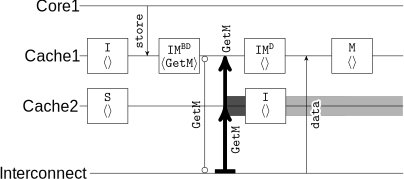
\includegraphics{\chapterdirectory/figure/store_seq_diagram_interference2_fixed.pdf}}
\end{center}
\caption{Expelling Cache Coherence Interference}
\label{fig:expelling-interference}
\end{figure}

\begin{example}[Expelling Interference]
Figure~\ref{fig:expelling-interference} shows an example of
expelling interference: Cache2, receiving
a demand for read-and-write access from Cache1, is forced to relinquish its
read-only copy of the memory element.
\end{example}

An expelling interference has an impact on the very first next instruction that
is either a \storeinstr{} or a \loadinstr{} (not \evictinstr{}), and not any
future instructions.

As with the previous type of coherence interference, detection of expelling
interference is done by annotating the coherence protocol. This time, the
annotation is done on transitions which make a memory element move from a
coherence state in which \loadinstr{} is a \hitact{} to one where it is not.
Detection of expelling interference that affected the program's run-time is also
done by using \lstinline!cache_local_address_infos! to keep track of which
memory elements have been affected by an expelling interference since they were
last accessed. The interference is considered to have had an impact on execution
time if either \loadinstr{} or \storeinstr{} occurs on a memory element
currently marked as having been forcefully evicted. This may result in
over-pessimism, as the \storeinstr{} might not have been a \hitact{} regardless
(e.g.~expelling interference occurring in the \texttt{S} state, followed by
\storeinstr{}).

\subsection{Protocol Annotations}
\begin{figure}[hbt!]
\begin{center}
%\scalebox{0.8}[0.8]{%
\begin{subfigure}{0.325\linewidth}
\resizebox{\linewidth}{!}{\input{\chapterdirectory/figure/msi_interference}}
\caption{MSI}
\label{fig:msi-interference}
\end{subfigure}
\begin{subfigure}{0.325\linewidth}
\resizebox{\linewidth}{!}{\input{\chapterdirectory/figure/mesi_interference}}
\caption{MESI}
\label{fig:mesi-interference}
\end{subfigure}
\begin{subfigure}{0.325\linewidth}
\resizebox{\linewidth}{!}{\begin{tabular}{|l||c|c|c|}
 \hline

 \textbf{State}
 & \multicolumn{3}{c|}{\textbf{Received Query}}
 \\

%%%%%%%%%%%%%%%%%%%%%%%%%%%%%%%%%%%%%%%%%%%%%%%%%%%%%%%%%%%%%%%%%%%%%%%%%%%%%%%%
 & \texttt{GetS} & \texttt{GetM} & \texttt{PutM}
 \\
 \hline

%%%%%%%%%%%%%%%%%%%%%%%%%%%%%%%%%%%%%%%%%%%%%%%%%%%%%%%%%%%%%%%%%%%%%%%%%%%%%%%%
 \texttt{I}

 & \cellcolor{olive!80}\texttt{Mi.}
 & \cellcolor{olive!80}\texttt{Mi.}
 & \cellcolor{olive!80}\texttt{Mi.}
 \\
 \hline

%%%%%%%%%%%%%%%%%%%%%%%%%%%%%%%%%%%%%%%%%%%%%%%%%%%%%%%%%%%%%%%%%%%%%%%%%%%%%%%%
 \texttt{IF\textsuperscript{BD}}

 & \cellcolor{olive!80}\texttt{Mi.}
 & \cellcolor{olive!80}\texttt{Mi.}
 & \cellcolor{olive!80}\texttt{Mi.}
 \\
 \hline

%%%%%%%%%%%%%%%%%%%%%%%%%%%%%%%%%%%%%%%%%%%%%%%%%%%%%%%%%%%%%%%%%%%%%%%%%%%%%%%%
 \texttt{IF\textsuperscript{B}}

 & \cellcolor{olive!80}\texttt{Mi.}
 & \cellcolor{olive!80}\texttt{Mi.}
 & \cellcolor{black!40}
 \\
 \hline

%%%%%%%%%%%%%%%%%%%%%%%%%%%%%%%%%%%%%%%%%%%%%%%%%%%%%%%%%%%%%%%%%%%%%%%%%%%%%%%%
 \texttt{IEoF\textsuperscript{D}}

 & \cellcolor{olive!80}\texttt{Mi.}
 & \cellcolor{orange!60}\texttt{Ex.}
 & \cellcolor{black!40}
 \\
 \hline

%%%%%%%%%%%%%%%%%%%%%%%%%%%%%%%%%%%%%%%%%%%%%%%%%%%%%%%%%%%%%%%%%%%%%%%%%%%%%%%%
 \texttt{IS\textsuperscript{D}}

 & \cellcolor{olive!80}\texttt{Mi.}
 & \cellcolor{orange!60}\texttt{Ex.}
 & \cellcolor{black!40}
 \\
 \hline

%%%%%%%%%%%%%%%%%%%%%%%%%%%%%%%%%%%%%%%%%%%%%%%%%%%%%%%%%%%%%%%%%%%%%%%%%%%%%%%%
 \texttt{IS\textsuperscript{D}I}

 % GetS/GetM/PutM
 & \cellcolor{olive!80}\texttt{Mi.}
 & \cellcolor{olive!80}\texttt{Mi.}
 & \cellcolor{black!40}
 \\
 \hline

%%%%%%%%%%%%%%%%%%%%%%%%%%%%%%%%%%%%%%%%%%%%%%%%%%%%%%%%%%%%%%%%%%%%%%%%%%%%%%%%
 \texttt{IM\textsuperscript{BD}}

 & \cellcolor{olive!80}\texttt{Mi.}
 & \cellcolor{olive!80}\texttt{Mi.}
 & \cellcolor{olive!80}\texttt{Mi.}
 \\
 \hline

%%%%%%%%%%%%%%%%%%%%%%%%%%%%%%%%%%%%%%%%%%%%%%%%%%%%%%%%%%%%%%%%%%%%%%%%%%%%%%%%
 \texttt{IM\textsuperscript{B}}

 % GetS/GetM/PutM
 & \cellcolor{olive!80}\texttt{Mi.}
 & \cellcolor{olive!80}\texttt{Mi.}
 & \cellcolor{olive!80}\texttt{Mi.}
 \\
 \hline

%%%%%%%%%%%%%%%%%%%%%%%%%%%%%%%%%%%%%%%%%%%%%%%%%%%%%%%%%%%%%%%%%%%%%%%%%%%%%%%%
 \texttt{IM\textsuperscript{D}}

 & \cellcolor{blue!40}\texttt{De.}
 & \cellcolor{orange!60}\texttt{Ex.}
 & \cellcolor{black!40}
 \\
 \hline

%%%%%%%%%%%%%%%%%%%%%%%%%%%%%%%%%%%%%%%%%%%%%%%%%%%%%%%%%%%%%%%%%%%%%%%%%%%%%%%%
 \texttt{IM\textsuperscript{D}I}

 & \cellcolor{olive!80}\texttt{Mi.}
 & \cellcolor{olive!80}\texttt{Mi.}
 & \cellcolor{black!40}
 \\
 \hline

%%%%%%%%%%%%%%%%%%%%%%%%%%%%%%%%%%%%%%%%%%%%%%%%%%%%%%%%%%%%%%%%%%%%%%%%%%%%%%%%
 \texttt{IM\textsuperscript{D}S}

 & \cellcolor{olive!80}\texttt{Mi.}
 & \cellcolor{orange!60}\texttt{Ex.}
 & \cellcolor{black!40}
 \\
 \hline

%%%%%%%%%%%%%%%%%%%%%%%%%%%%%%%%%%%%%%%%%%%%%%%%%%%%%%%%%%%%%%%%%%%%%%%%%%%%%%%%
 \texttt{IM\textsuperscript{D}SI}

 & \cellcolor{olive!80}\texttt{Mi.}
 & \cellcolor{olive!80}\texttt{Mi.}
 & \cellcolor{black!40}
 \\
 \hline

%%%%%%%%%%%%%%%%%%%%%%%%%%%%%%%%%%%%%%%%%%%%%%%%%%%%%%%%%%%%%%%%%%%%%%%%%%%%%%%%
 \texttt{S}

 & \cellcolor{olive!80}\texttt{Mi.}
 & \cellcolor{orange!60}\texttt{Ex.}
 & \cellcolor{black!40}
 \\
 \hline

%%%%%%%%%%%%%%%%%%%%%%%%%%%%%%%%%%%%%%%%%%%%%%%%%%%%%%%%%%%%%%%%%%%%%%%%%%%%%%%%
 \texttt{F}

 & \cellcolor{olive!80}\texttt{Mi.}
 & \cellcolor{orange!60}\texttt{Ex.}
 & \cellcolor{black!40}
 \\
 \hline

%%%%%%%%%%%%%%%%%%%%%%%%%%%%%%%%%%%%%%%%%%%%%%%%%%%%%%%%%%%%%%%%%%%%%%%%%%%%%%%%
 \texttt{SM\textsuperscript{BD}}

 & \cellcolor{olive!80}\texttt{Mi.}
 & \cellcolor{orange!60}\texttt{Ex.}
 & \cellcolor{black!40}
 \\
 \hline

%%%%%%%%%%%%%%%%%%%%%%%%%%%%%%%%%%%%%%%%%%%%%%%%%%%%%%%%%%%%%%%%%%%%%%%%%%%%%%%%
 \texttt{FM\textsuperscript{B}}

 & \cellcolor{olive!80}\texttt{Mi.}
 & \cellcolor{olive!80}\texttt{Mi.}
 & \cellcolor{black!40}
 \\
 \hline

%%%%%%%%%%%%%%%%%%%%%%%%%%%%%%%%%%%%%%%%%%%%%%%%%%%%%%%%%%%%%%%%%%%%%%%%%%%%%%%%
 \texttt{SM\textsuperscript{B}}

 & \cellcolor{olive!80}\texttt{Mi.}
 & \cellcolor{olive!80}\texttt{Mi.}
 & \cellcolor{black!40}
 \\
 \hline

%%%%%%%%%%%%%%%%%%%%%%%%%%%%%%%%%%%%%%%%%%%%%%%%%%%%%%%%%%%%%%%%%%%%%%%%%%%%%%%%
 \texttt{SM\textsuperscript{D}}

 & \cellcolor{blue!40}\texttt{De.}
 & \cellcolor{orange!60}\texttt{Ex.}
 & \cellcolor{black!40}
 \\
 \hline

%%%%%%%%%%%%%%%%%%%%%%%%%%%%%%%%%%%%%%%%%%%%%%%%%%%%%%%%%%%%%%%%%%%%%%%%%%%%%%%%
 \texttt{SM\textsuperscript{D}I}

 & \cellcolor{olive!80}\texttt{Mi.}
 & \cellcolor{olive!80}\texttt{Mi.}
 & \cellcolor{black!40}
 \\
 \hline

%%%%%%%%%%%%%%%%%%%%%%%%%%%%%%%%%%%%%%%%%%%%%%%%%%%%%%%%%%%%%%%%%%%%%%%%%%%%%%%%
 \texttt{SM\textsuperscript{D}S}

 & \cellcolor{olive!80}\texttt{Mi.}
 & \cellcolor{orange!60}\texttt{Ex.}
 & \cellcolor{black!40}
 \\
 \hline

%%%%%%%%%%%%%%%%%%%%%%%%%%%%%%%%%%%%%%%%%%%%%%%%%%%%%%%%%%%%%%%%%%%%%%%%%%%%%%%%
 \texttt{SM\textsuperscript{D}SI}

 & \cellcolor{olive!80}\texttt{Mi.}
 & \cellcolor{olive!80}\texttt{Mi.}
 & \cellcolor{black!40}
 \\
 \hline

%%%%%%%%%%%%%%%%%%%%%%%%%%%%%%%%%%%%%%%%%%%%%%%%%%%%%%%%%%%%%%%%%%%%%%%%%%%%%%%%
 \texttt{M}

 & \cellcolor{blue!40}\texttt{De.}
 & \cellcolor{orange!60}\texttt{Ex.}
 & \cellcolor{black!40}
 \\
 \hline

%%%%%%%%%%%%%%%%%%%%%%%%%%%%%%%%%%%%%%%%%%%%%%%%%%%%%%%%%%%%%%%%%%%%%%%%%%%%%%%%
 \texttt{MI\textsuperscript{B}}

 & \cellcolor{orange!60}\texttt{Ex.}
 & \cellcolor{orange!60}\texttt{Ex.}
 & \cellcolor{black!40}
 \\
 \hline

%%%%%%%%%%%%%%%%%%%%%%%%%%%%%%%%%%%%%%%%%%%%%%%%%%%%%%%%%%%%%%%%%%%%%%%%%%%%%%%%
 \texttt{II\textsuperscript{B}}

 & \cellcolor{olive!80}\texttt{Mi.}
 & \cellcolor{olive!80}\texttt{Mi.}
 & \cellcolor{olive!80}\texttt{Mi.}
 \\
 \hline

%%%%%%%%%%%%%%%%%%%%%%%%%%%%%%%%%%%%%%%%%%%%%%%%%%%%%%%%%%%%%%%%%%%%%%%%%%%%%%%%
 \texttt{E}

 & \cellcolor{blue!40}\texttt{De.}
 & \cellcolor{orange!60}\texttt{Ex.}
 & \cellcolor{black!40}
 \\
 \hline

%%%%%%%%%%%%%%%%%%%%%%%%%%%%%%%%%%%%%%%%%%%%%%%%%%%%%%%%%%%%%%%%%%%%%%%%%%%%%%%%
 \texttt{IE\textsuperscript{B}}
 & \cellcolor{olive!80}\texttt{Mi.}
 & \cellcolor{olive!80}\texttt{Mi.}
 & \cellcolor{olive!80}\texttt{Mi.}
 \\
 \hline

%%%%%%%%%%%%%%%%%%%%%%%%%%%%%%%%%%%%%%%%%%%%%%%%%%%%%%%%%%%%%%%%%%%%%%%%%%%%%%%%
 \texttt{EI\textsuperscript{B}}
 & \cellcolor{orange!60}\texttt{Ex.}
 & \cellcolor{orange!60}\texttt{Ex.}
 & \cellcolor{black!40}
 \\
 \hline

%%%%%%%%%%%%%%%%%%%%%%%%%%%%%%%%%%%%%%%%%%%%%%%%%%%%%%%%%%%%%%%%%%%%%%%%%%%%%%%%
 \texttt{FI\textsuperscript{B}}

 & \cellcolor{olive!80}\texttt{Mi.}
 & \cellcolor{olive!80}\texttt{Mi.}
 & \cellcolor{black!40}
 \\
 \hline

\end{tabular}%
}
\caption{MESIF}
\label{fig:mesif-interference}
\end{subfigure}
%}
\\
\vspace{1em}
Interference Type:
\begin{tabular}{|lll|}
\hline
\cellcolor{olive!80}Minor &
\cellcolor{orange!60}Expelling &
\cellcolor{blue!40}Demoting\\
\hline
\end{tabular}\\
\end{center}
\caption{Interference Annotations}
\label{fig:interference_annotations}
\end{figure}

Figure~\ref{fig:interference_annotations} shows the proposed interference
annotation for the 3 coherence protocols presented in this thesis: MSI, MESI,
and MESIF.

\paragraph{Explanations for the \textit{Demoting} annotations:}
\begin{itemize}
\item
   Receiving \getsquery{} external query for a memory element in the
   \texttt{IM\textsuperscript{D}} state will prevent the cache from keeping the
   write permissions after the current \storeinstr{} for this memory element
   completes, hence the \textit{Demoting} annotations.
\item
   In the \texttt{M} and \texttt{E} states, observing a \getsquery{} external
   query will result in the immediate loss of writing permissions for that
   memory element, which is why these transitions are marked with
   \textit{Demoting} annotations.
\end{itemize}

\paragraph{Explanations for the \textit{Expelling} annotations:}
\begin{itemize}
\item
   Observing a \getmquery{} query for a memory element in the
   \texttt{IS\textsuperscript{D}}, \texttt{IM\textsuperscript{D}},
   \texttt{SM\textsuperscript{D}}, \texttt{IEoS\textsuperscript{D}},
   \texttt{IEoF\textsuperscript{D}}, or \texttt{SM\textsuperscript{D}S} state
   leads to states that ensure the memory element is evicted once this cache's
   current transaction for the memory element is completed. They are thus
   annotated as \textit{Expelling} interference.
\item
   Similarly, receiving a \getmquery{} query for a memory element in the
   \texttt{S}, \texttt{M}, \texttt{E}, or \texttt{F} leads to that memory being
   immediately evicted (and thus are also annotated as \textit{Expelling}
   interference).
\item
   The \textit{Expelling} interference annotations on the transitions for
   \texttt{MI\textsuperscript{B}} and \texttt{EI\textsuperscript{B}} come from
   the fact that, until it observes any query for that memory element, the cache
   still has both read and write permissions. These states were reached because
   the cache is already evicting the memory element, which makes considering its
   eviction an interference something that can be argued against. I chose to
   consider the permissions for future requests and not the result of past ones,
   hence the annotation.
\end{itemize}

\begin{example}[Impact of External Queries on the Model from Section~\ref{sec:analysis:demo_model}]
As previously stated, the direct application of the analyses proposed in this
section are unlikely to produce exploitable results. Nevertheless, in order to
illustrate the concepts, this subsection proposes an analysis of the queries
generated by the example of Section~\ref{sec:analysis:demo_model}.

By using counters for occurrences of potential interference and those which
had an impact, using model checking to obtain extrema may provide results
that can be compared to those from Section~\ref{sec:analysis:hit_and_miss}.
For example, the maximum number of occurrences for minor interference
related to the memory element at address \lstinline!target_addr! on Cache1, the
following query can be used:~~\\
\lstinline!sup: Cache1.cache_local_address_infos[target_addr].potential_interference_count[INTERFERENCE_MINOR]!.


\begin{figure}[hbt!]
\begin{center}
\begin{subfigure}[t]{\textwidth}
\centering
\begin{tabular}{|c|c|c|c|c|c|c|}
\cline{2-7}
\multicolumn{1}{c|}{} &
\multicolumn{3}{c|}{Cache1} &
\multicolumn{3}{c|}{Cache2} \\
\multicolumn{1}{c|}{} & Minor & Demoting & Expelling & Minor & Demoting &
Expelling\\
\hline
Address 1 & 1 (-) & 1 (1) & 2 (1) & 1 (-) & 1 (1) & 2 (2)\\
\hline
Address 2 & 0 (-) & 1 (1) & 2 (2) & 1 (-) & 1 (0) & 2 (1)\\
\hline
Address 3 & 1 (-) & 0 (0) & 1 (0) & 0 (-) & 1 (1) & 0 (0)\\
\hline
\end{tabular}
\caption{Maximum}
\label{fig:analyzing:maximum_interference}
\end{subfigure}
\\\vspace{1em}
\begin{subfigure}[t]{\textwidth}
\centering
\begin{tabular}{|c|c|c|c|c|c|c|}
\cline{2-7}
\multicolumn{1}{c|}{} &
\multicolumn{3}{c|}{Cache1} &
\multicolumn{3}{c|}{Cache2} \\
\multicolumn{1}{c|}{} & Minor & Demoting & Expelling & Minor & Demoting &
Expelling\\
\hline
Address 1 & 0 (-) & 1 (1) & 1 (0) & 0 (-) & 0 (0) & 2 (1)\\
\hline
Address 2 & 0 (-) & 0 (0) & 1 (1) & 1 (-) & 0 (0) & 1 (1)\\
\hline
Address 3 & 1 (-) & 0 (0) & 1 (0) & 0 (-) & 1 (1) & 0 (0)\\
\hline
\end{tabular}
\caption{Minimum}
\label{fig:analyzing:minimum_interference}
\end{subfigure}
\end{center}
\caption{Interference occurrence count extrema for each memory element, in
parenthesis is the number of occurrences that had an impact on execution times}
\label{fig:analyzing:interference_extrema}
\end{figure}

Figure~\ref{fig:analyzing:interference_extrema} shows the number of occurrences
of each interference category, for each cache and each address. Two values are
provided: the number of occurrences themselves and, in parenthesis, the number
of occurrences that had an impact on execution time. As indicated in
Section~\ref{sec:analysis:minor_interference}, the model is unable
to determine which occurrences of minor interference had an impact on execution
time, hence the lack of number for that category in the figure.

The results of Example~\ref{ex:analysis:hit_miss} showed that the interference
affected Cache2 only for the memory element at address 2, and that it led to
one of two instructions being a cache hit in every execution where the other
was a miss. The results from Figure~\ref{fig:analyzing:interference_extrema}
offer some further details, by showing that this is due to an expelling
interference. Indeed, there is no variation between
Figure~\ref{fig:analyzing:maximum_interference} and
Figure~\ref{fig:analyzing:minimum_interference} for the number of occurrences
of interference that had an impact on address 2.

Surprisingly, there is a variation for the number of expelling interference
that can have an impact on address 1 in Cache2. This is not visible in the
categorization from Figure~\ref{fig:analysis:demo_chara_prog2}, as all accesses
made to address 1 are either \textit{always-hit} or \textit{always-miss}. The
reason for the extra interference not preventing this categorization is that,
in effect, it had not impact. Indeed, performing a \storeinstr{} on a memory
element in the \texttt{Invalid} or \texttt{Shared} state both result in a cache
miss. However, if an external query evicted the memory element while it was in
the \texttt{Shared} state, this forced eviction is still considered as having
had an impact on the \storeinstr{} by the model.

Looking at the results for Cache1 and the address 1, the difference between
Figure~\ref{fig:analyzing:maximum_interference} and
Figure~\ref{fig:analyzing:minimum_interference} only indicates a single
expelling interference not always occurring. In
Figure~\ref{fig:analysis:demo_chara_prog1} however, the categorization for
accesses to the address 1 failed on two instructions. From the fact that there
is only this single expelling interference that can vary in all executions,
these two instructions are either both affected or neither is. In effect, they
are either both a cache hit, or both a cache miss.

The results for address 2 on the Cache1 show that there are two impactful
instances of interference that may or may not happen in executions. Since the
category of interference are not the same for the two instances, the results
presented here are insufficient to determine a meaningful pattern. To resolve
this, further model checking queries would have to be made in order to see if
the two interference occurrences are somehow related.
\end{example}

In order to render the analysis of query interference more exploitable, the
user would need to be made aware both with instruction was affected and which
instruction generated the query. This is achieved in the next Section.
